% =====================================================================
%  OSDA / SandboxSentinel -- Project Report
%
%  Compile with:   pdflatex osda-report.tex
%                  pdflatex osda-report.tex     (run twice, for the ToC)
%
%  SCREENSHOTS: drop your two captures into  docs/figures/  as
%      figures/case-safe.png      -- a SAFE verdict run
%      figures/case-unsafe.png    -- a SUSPICIOUS/MALICIOUS verdict run
%  Until those files exist the document still compiles and renders a
%  labelled placeholder box in their place (see \screenshot below).
% =====================================================================
\documentclass[11pt,a4paper]{article}

\usepackage[T1]{fontenc}
\usepackage[utf8]{inputenc}
\usepackage{lmodern}
\usepackage[margin=1in]{geometry}
\usepackage{graphicx}
\usepackage{xcolor}
\usepackage{booktabs}
\usepackage{longtable}
\usepackage{listings}
\usepackage{enumitem}
\usepackage{caption}
\usepackage{tikz}
\usepackage{float}
\usepackage[hidelinks]{hyperref}

\usetikzlibrary{arrows.meta, positioning, calc}

% ---------------------------------------------------------------- colours
\definecolor{codebg}{RGB}{247,247,249}
\definecolor{codekw}{RGB}{0,85,150}
\definecolor{codestr}{RGB}{150,40,40}
\definecolor{codecmt}{RGB}{100,110,100}
\definecolor{rulegrey}{RGB}{200,200,205}
\definecolor{boxsafe}{RGB}{30,120,60}
\definecolor{boxbad}{RGB}{170,40,40}

% ---------------------------------------------------------------- listings
\lstdefinestyle{osda}{
  backgroundcolor=\color{codebg},
  basicstyle=\ttfamily\scriptsize,
  keywordstyle=\color{codekw}\bfseries,
  stringstyle=\color{codestr},
  commentstyle=\color{codecmt}\itshape,
  numberstyle=\tiny\color{gray},
  breaklines=true,
  breakatwhitespace=false,
  showstringspaces=false,
  frame=single,
  rulecolor=\color{rulegrey},
  framesep=4pt,
  xleftmargin=10pt,
  columns=fullflexible,
  keepspaces=true,
  upquote=true,
  tabsize=4,
}
\lstset{style=osda}
\lstdefinestyle{osdanum}{style=osda,numbers=left,numbersep=6pt}
\lstdefinestyle{term}{style=osda,language=,basicstyle=\ttfamily\scriptsize}

% ---------------------------------------------------------------- helpers
\newcommand{\code}[1]{\texttt{\small #1}}
\newcommand{\file}[1]{\texttt{\small #1}}

% Screenshot with graceful placeholder.
% #1 image path   #2 caption   #3 label   #4 placeholder hint text
\newcommand{\screenshot}[4]{%
  \begin{figure}[H]
  \centering
  \IfFileExists{#1}{%
    \includegraphics[width=0.95\textwidth]{#1}%
  }{%
    \begin{tikzpicture}
      \draw[dashed, rulegrey, line width=1pt, fill=codebg]
        (0,0) rectangle (0.95\textwidth, 0.46\textwidth);
      \node[align=center, text width=0.78\textwidth]
        at (0.475\textwidth, 0.23\textwidth)
        {\ttfamily\small [ SCREENSHOT PLACEHOLDER ]\\[8pt]
         \ttfamily\footnotesize #1\\[10pt]
         \rmfamily\small #4};
    \end{tikzpicture}%
  }
  \caption{#2}
  \label{#3}
  \end{figure}}

% =====================================================================
\title{\textbf{OSDA / SandboxSentinel}\\[6pt]
\large An Automated Dynamic Analysis Sandbox using Docker Isolation,\\
eBPF Kernel Tracing and Process-Tree Correlation}
\author{Yashwant Gokul}
\date{\today}

\begin{document}
\maketitle

\begin{abstract}
\noindent
OSDA (Operating System Dynamic Analysis), developed under the working name
\emph{SandboxSentinel}, is an automated dynamic analysis platform that executes
untrusted Python (\code{.py}) and shell (\code{.sh}) scripts inside a disposable
Docker container while observing their behaviour from the host kernel. Instead of
installing an agent inside the guest --- which the sample could detect, disable or
subvert --- OSDA attaches eBPF probes to Linux scheduler and syscall tracepoints on
the host and reconstructs the sandbox's activity from the outside. Captured
\code{execve} invocations (including command-line arguments), fork and exit events,
and \code{inotify} filesystem events are funnelled through a single event queue,
attributed to the sandbox by \emph{PID namespace inode}, correlated into a process
hierarchy, and finally scored by an explainable heuristic engine that emits a
0--100 risk score and a \textsc{safe}/\textsc{suspicious}/\textsc{malicious}
verdict together with the evidence that produced it. This report documents the
system's motivation, architecture, module-level design, heuristic rule catalogue,
the engineering problems encountered (notably argv truncation in \code{ctypes} and
PID-namespace mismatch under WSL2), two end-to-end case studies, the test strategy,
and the platform's known coverage limitations.
\end{abstract}

\tableofcontents
\newpage

% =====================================================================
\section{Introduction}

\subsection{Motivation}
Static inspection of a script --- reading it, grepping it, hashing it against a
reputation feed --- answers the question \emph{``what does this file look like?''}
It does not answer \emph{``what does this file do?''} A payload that assembles its
command line at runtime, decodes a base64 blob, or downloads its second stage from
a remote host reveals nothing useful to a static reader. Behaviour is only visible
during execution, and execution of an untrusted file is exactly what an analyst
cannot safely do on a workstation.

A sandbox resolves that tension: the file is allowed to run, but inside a container
whose filesystem, process namespace and lifetime are disposable, and under
instrumentation that records what it actually did. OSDA is such a sandbox, built
for scripts rather than for compiled binaries, and designed so that the
instrumentation lives entirely on the host side of the isolation boundary.

\subsection{Objectives}
\begin{enumerate}[leftmargin=*]
  \item \textbf{Isolated execution.} Run an arbitrary \code{.py} or \code{.sh} file
        in a short-lived Docker container with its own PID, mount and network
        namespaces, so that any side effects are confined and discarded.
  \item \textbf{Agentless observation.} Collect process telemetry from host-side
        eBPF tracepoints rather than from a cooperating process inside the guest.
  \item \textbf{Faithful attribution.} Separate the sandbox's processes from the
        host's background noise, even when the eBPF view and Docker's view do not
        share a PID numbering space.
  \item \textbf{Correlation.} Rebuild the parent/child execution lineage into a
        readable process tree rather than presenting a flat event log.
  \item \textbf{Explainable verdict.} Produce a bounded risk score and a verdict in
        which every point is traceable to a named rule and the exact command line
        that triggered it.
  \item \textbf{Honest reporting.} State the analysis's blind spots in the report
        itself, so a \textsc{safe} verdict is never mistaken for a guarantee.
\end{enumerate}

\subsection{Scope and non-goals}
OSDA analyses interpreted scripts in two languages and observes three classes of
behaviour: process execution, workspace filesystem mutation, and network intent
inferred from command-line arguments. It is explicitly \emph{not} a packet-capture
platform, not a system-call-complete tracer, not a signature or YARA engine, and
not a verdict authority. The heuristics describe what was observed in one execution
of one sample on one input; they do not generalise to claims about the file's safety.

% =====================================================================
\section{Background}

\subsection{Dynamic analysis and the agent problem}
Classical sandboxes (Cuckoo and its descendants) place an agent inside the guest to
hook API calls and report back. The agent is powerful --- it sees userland calls in
full detail --- but it is also inside the blast radius. Malware can enumerate it,
kill it, or simply behave differently when it is present. Host-side kernel
instrumentation inverts this: the observer sits below the isolation boundary, in a
privilege domain the sample cannot reach, and the guest contains no OSDA code at all.

\subsection{eBPF tracepoints}
eBPF allows verified programs to be loaded into the running kernel and attached to
instrumentation points. OSDA uses two families:

\begin{itemize}[leftmargin=*]
  \item \textbf{Scheduler tracepoints} --- \code{sched:sched\_process\_exec},
        \code{sched:sched\_process\_fork} and \code{sched:sched\_process\_exit}.
        These fire for every process in the system that respectively replaces its
        image, creates a child, or terminates. They are stable, cheap, and
        unavoidable: a process cannot execute without passing through
        \code{sched\_process\_exec}.
  \item \textbf{Syscall tracepoints} --- \code{syscalls:sys\_enter\_execve} and
        \code{syscalls:sys\_exit\_execve}. The scheduler exec tracepoint reports
        \emph{that} an exec happened and under which \code{comm}, but not the
        argument vector. The argument vector is only reachable from user memory at
        syscall entry, so OSDA reads it there, stashes it in a BPF hash keyed by
        \code{pid\_tgid}, and joins it to the scheduler event that follows.
\end{itemize}

\subsection{Namespaces as the unit of attribution}
A tracepoint on the host fires for \emph{every} process on the machine. The sandbox
is a subset of those, and the system needs a reliable membership test. Docker
reports the container's root PID in its own numbering space; eBPF reports PIDs in
the initial namespace. When the Docker daemon itself runs inside a nested PID
namespace --- which is exactly the situation under WSL2 --- those two numbers are not
comparable, and ancestry walks rooted at Docker's number collapse. OSDA therefore
attributes events by the \emph{inode number of the PID namespace}, read once from
\file{/proc/<root\_pid>/ns/pid}. An inode identifies the same namespace object from
every numbering space, which makes the membership test namespace-nesting agnostic.
This design decision is examined in detail in Section~\ref{sec:nsfix}.

% =====================================================================
\section{System Architecture}

\subsection{Overview}
OSDA is a producer/consumer pipeline. Two independent monitors produce
\code{Event} objects into a shared \code{queue.Queue}; one consumer thread drains
the queue and fans each event out to both the report generator (which keeps the raw
log) and the process-tree correlator (which keeps the structure). When the container
exits, the correlator's completed tree and the raw event list are handed to the
security evaluator, whose findings are then rendered inline in the report.

\begin{figure}[H]
\centering
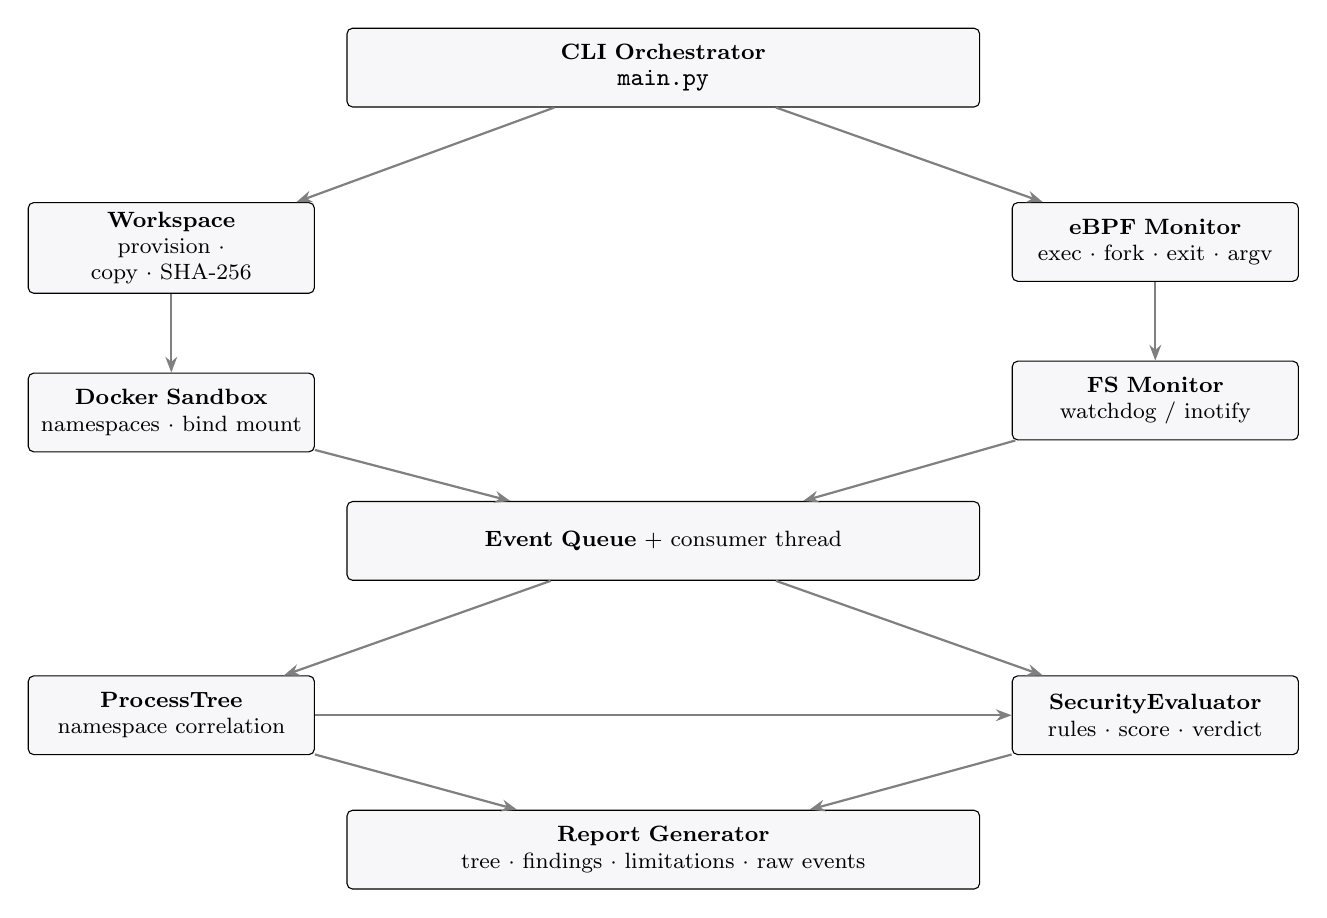
\begin{tikzpicture}[
  node distance=10mm and 12mm,
  box/.style={draw, rounded corners=2pt, align=center, font=\footnotesize,
              minimum height=10mm, text width=34mm, fill=codebg},
  wide/.style={box, text width=78mm},
  arr/.style={-{Stealth[length=2mm]}, thick, gray}]

  \node[wide] (cli) {\textbf{CLI Orchestrator}\\\file{main.py}};

  \node[box, below left=12mm and 4mm of cli] (ws)
    {\textbf{Workspace}\\provision $\cdot$ copy $\cdot$ SHA-256};
  \node[box, below right=12mm and 4mm of cli] (ebpf)
    {\textbf{eBPF Monitor}\\exec $\cdot$ fork $\cdot$ exit $\cdot$ argv};

  \node[box, below=of ws] (cont)
    {\textbf{Docker Sandbox}\\namespaces $\cdot$ bind mount};
  \node[box, below=of ebpf] (fs)
    {\textbf{FS Monitor}\\watchdog / inotify};

  \node[wide, below=12mm of $(cont)!0.5!(fs)$] (q)
    {\textbf{Event Queue} $+$ consumer thread};

  \node[box, below left=12mm and 4mm of q] (tree)
    {\textbf{ProcessTree}\\namespace correlation};
  \node[box, below right=12mm and 4mm of q] (eval)
    {\textbf{SecurityEvaluator}\\rules $\cdot$ score $\cdot$ verdict};

  \node[wide, below=12mm of $(tree)!0.5!(eval)$] (rep)
    {\textbf{Report Generator}\\tree $\cdot$ findings $\cdot$ limitations $\cdot$ raw events};

  \draw[arr] (cli)  -- (ws);
  \draw[arr] (cli)  -- (ebpf);
  \draw[arr] (ws)   -- (cont);
  \draw[arr] (ebpf) -- (fs);
  \draw[arr] (cont) -- (q);
  \draw[arr] (fs)   -- (q);
  \draw[arr] (q)    -- (tree);
  \draw[arr] (q)    -- (eval);
  \draw[arr] (tree) -- (eval);
  \draw[arr] (tree) -- (rep);
  \draw[arr] (eval) -- (rep);
\end{tikzpicture}
\caption{OSDA data flow. Monitors produce events on the host side of the isolation
boundary; the container itself contains no OSDA code.}
\label{fig:arch}
\end{figure}

\subsection{Repository layout}
\begin{lstlisting}[style=term]
osda/
  correlate/
    process_tree.py   # parent/child correlation, namespace membership, ASCII render
    evaluator.py      # heuristic rules, risk score, verdict
  internal/
    models.py         # Event dataclass and EventType enum
  monitors/
    ebpf_process.py   # BPF C program, perf-buffer polling, argv decoding
    fs_monitor.py     # watchdog observer over the mounted workspace
  report/
    generator.py      # textual report assembly, ANSI verdict colouring
  sandbox/
    container.py      # Docker lifecycle (pull, create, start, wait, cleanup)
    workspace.py      # isolated working directory, SHA-256 snapshotting
  tests/
    test_evaluator.py # scoring, attribution and rendering tests
    test_argv.py      # argv decoding tests (no kernel required)
  main.py             # CLI entrypoint and pipeline orchestration
  Dockerfile          # shell-analysis image (debian:stable-slim + utilities)
  requirements.txt    # docker==7.1.0, watchdog==4.0.2
  sample.py           # benign reference sample
  suspicious.sh       # sample exercising subshell + download behaviour
\end{lstlisting}

% =====================================================================
\section{Module Design}

\subsection{Event model (\file{internal/models.py})}
A single \code{Event} dataclass carries every observation, with optional fields per
category. Keeping one type means the queue, the consumer and the report need no
polymorphism.

\begin{table}[H]
\centering\footnotesize
\begin{tabular}{@{}llp{74mm}@{}}
\toprule
\textbf{Field} & \textbf{Type} & \textbf{Purpose} \\
\midrule
\code{analysis\_id}    & \code{str}  & Run identifier, stamped by the consumer \\
\code{container\_id}   & \code{str}  & Docker container the event belongs to \\
\code{timestamp}       & \code{float}& Host wall-clock time, used for ordering \\
\code{type}            & \code{EventType} & One of nine event kinds \\
\code{pid}, \code{ppid}& \code{int}  & Process identity (initial namespace) \\
\code{process\_name}   & \code{str}  & Kernel \code{comm}, 16 bytes \\
\code{file\_path}      & \code{str}  & Workspace-relative path, filesystem events \\
\code{remote\_address}, \code{remote\_port} & & Reserved for direct network capture \\
\code{argv}            & \code{list[str]} & Decoded argument vector, exec events \\
\code{argv\_truncated} & \code{bool} & Set when argv exceeded capture limits \\
\code{pid\_ns}         & \code{int}  & \textbf{PID namespace inode --- the attribution key} \\
\bottomrule
\end{tabular}
\caption{The \code{Event} dataclass.}
\end{table}

\code{EventType} enumerates \code{PROCESS\_EXEC}, \code{PROCESS\_FORK},
\code{PROCESS\_EXIT}, \code{FILE\_CREATE}, \code{FILE\_MODIFY},
\code{FILE\_DELETE}, \code{FILE\_CHMOD} and \code{NETWORK\_CONNECT}.

\subsection{Workspace isolation (\file{sandbox/workspace.py})}
Each run gets \file{./sandboxes/<analysis\_id>/workspace/}, created before the
container and recursively removed after it. The target file is copied in with
\code{shutil.copy2} (preserving mode, so an executable stays executable), and the
directory is bind-mounted at \file{/workspace} inside the container. The class also
provides \code{hash\_file} (streaming SHA-256 in 4\,KiB blocks) and
\code{snapshot}, which walks the tree and returns a
\code{\{relative\_path: sha256\}} mapping, tolerating files that vanish mid-walk.

\subsection{Container lifecycle (\file{sandbox/container.py})}
A thin wrapper over the \code{docker} SDK with a deliberate two-phase start:

\begin{lstlisting}[language=Python,style=osdanum]
def create(self, cmd: str):
    abs_workspace = os.path.abspath(self.workspace_path)
    self.container = self.client.containers.create(
        self.image,
        command=cmd,
        volumes={abs_workspace: {'bind': '/workspace', 'mode': 'rw'}},
        detach=True,
        tty=True
    )
    self.container_id = self.container.id
\end{lstlisting}

Separating \code{create} from \code{start} is what makes agentless capture possible:
the container ID exists --- so the filesystem monitor can be wired up, and the eBPF
monitor is already polling --- before a single instruction of the sample has run.
Starting and instrumenting in one step would race, and the first \code{execve} would
be lost. Images are selected by extension: \code{python:3.12-slim} for \code{.py},
and the locally built \code{sandboxsentinel-shell:latest} for \code{.sh}.

\subsection{eBPF process monitor (\file{monitors/ebpf\_process.py})}
This is the core of the system. A BPF C program is compiled at runtime by BCC and
attached to five tracepoints. Three structures back it: a \code{BPF\_PERF\_OUTPUT}
channel to userspace, a \code{BPF\_HASH} (\code{exec\_args}) that carries argv from
syscall entry to the scheduler event, and a \code{BPF\_PERCPU\_ARRAY}
(\code{exec\_scratch}) used as scratch space, because the event struct is far larger
than the 512-byte BPF stack allows.

\begin{lstlisting}[language=C,style=osdanum]
struct event_t {
    u32 pid;
    u32 ppid;
    u32 type;                         // 1=EXEC, 2=FORK, 3=EXIT
    char comm[TASK_COMM_LEN];
    char argv[ARG_COUNT * ARG_SIZE];  // flattened: BCC cannot decode 2-D arrays
    u32 argv_truncated;
    u32 pid_ns;
};
\end{lstlisting}

\paragraph{Argument capture.} At \code{sys\_enter\_execve} the program unrolls over
up to \code{ARG\_COUNT} $=8$ pointers in the user \code{argv} array, copying each
string with \code{bpf\_probe\_read\_user\_str} into a fixed \code{ARG\_SIZE} $=96$
byte slot. A return length of \code{ARG\_SIZE} or more means the argument was
clipped, and a non-null pointer at index \code{ARG\_COUNT} means arguments were
dropped entirely; either sets \code{argv\_truncated}, which the report later
surfaces as a coverage limitation rather than silently hiding.

\paragraph{Joining argv to the exec.} At \code{sched\_process\_exec} the saved entry
is looked up by \code{pid\_tgid}. If present it is used and deleted; if absent ---
which happens for \code{execveat}, or when the monitor started mid-exec --- a
cleared scratch struct is submitted with \code{argv\_truncated} already set, so the
event is never silently argv-less. The namespace inode is read from the task struct:

\begin{lstlisting}[language=C,style=osdanum]
struct task_struct *task = (struct task_struct *)bpf_get_current_task();
event->ppid   = task->real_parent->tgid;
event->pid_ns = task->nsproxy->pid_ns_for_children->ns.inum;
\end{lstlisting}

\paragraph{Userspace side.} A daemon thread calls \code{perf\_buffer\_poll} on a
100\,ms timeout; \code{stop()} polls once more so that events still in flight when
the container exits are drained rather than dropped. If the \code{bcc} module is
absent the monitor degrades to a no-op with a warning, which lets the rest of the
pipeline (and the whole test suite) run on non-Linux hosts. The module also appends
\file{/usr/lib/python3/dist-packages} to \code{sys.path}, because
\code{python3-bpfcc} is a distribution package that a virtualenv would otherwise not
see.

\subsection{Filesystem monitor (\file{monitors/fs\_monitor.py})}
A \code{watchdog} \code{Observer} watches the mounted workspace recursively and
translates \code{on\_created}, \code{on\_modified}, \code{on\_deleted} and
\code{on\_moved} into \code{FILE\_CREATE}, \code{FILE\_MODIFY} and
\code{FILE\_DELETE} events, with paths made relative to the workspace root. A move
is recorded as a delete, a documented simplification. Directory events are ignored.
Because the observer is attached to the \emph{host} side of the bind mount, writes
from inside the container are visible without any guest cooperation --- but equally,
only writes to \file{/workspace} are visible at all.

\subsection{Process-tree correlation (\file{correlate/process\_tree.py})}
\code{ProcessTree} maintains \code{\{pid: ProcessNode\}} and answers three
questions: which PIDs belong to the sandbox, which of those are entry points, and
how do they render. Membership prefers namespace identity and falls back to
ancestry:

\begin{lstlisting}[language=Python,style=osdanum]
def sandbox_pids(self):
    if self.container_pid_ns is not None:
        return {pid for pid, node in self.nodes.items()
                if node.pid_ns == self.container_pid_ns}
    pids = {self.root_pid} if self.root_pid and self.root_pid > 0 else set()
    while True:
        descendants = {pid for pid, node in self.nodes.items() if node.ppid in pids}
        if descendants <= pids:
            return pids
        pids.update(descendants)
\end{lstlisting}

A fork for an as-yet-unknown parent synthesises an \code{unknown\_parent}
placeholder rather than dropping the child, so a subtree is never orphaned by event
ordering. \code{root\_pids} returns sandbox PIDs whose parent lies outside the
sandbox --- the entry points --- and \code{render} walks down from those with a
\code{visited} set for cycle safety, appending a \code{[FLAGGED: rule, \dots]}
suffix to any node the evaluator implicated. The findings are thus visible
\emph{in} the structure, not only in a separate list.

\subsection{Security evaluator (\file{correlate/evaluator.py})}
The evaluator takes the completed tree and the raw event list and emits an
\code{Evaluation(score, verdict, findings, limitations)}. Three design rules govern
it:

\begin{enumerate}[leftmargin=*]
  \item \textbf{Scope.} Only events whose PID is in \code{sandbox\_pids()} are
        considered (plus PID-less filesystem events belonging to this analysis).
        Host noise picked up by the tracepoints cannot influence the score.
  \item \textbf{Deduplication.} Findings are keyed on \code{(rule, pid)}, so a loop
        that runs \code{curl} two hundred times scores once. Without this,
        repetition alone would reach a \textsc{malicious} verdict.
  \item \textbf{Bounded score.} The total is \code{min(100, sum(points))}, keeping
        the scale meaningful at the top end.
\end{enumerate}

Each exec event is normalised --- \code{PurePosixPath(argv[0]).name} for the
basename, \code{shlex.join(argv)} for the human-readable command --- and then
matched against the rule catalogue of Section~\ref{sec:rules}. One rule is stateful:
the \emph{dropper} rule tracks download targets from \code{-o}/\code{-O}/\code{--output}
arguments, notes which of those are later passed to \code{chmod +x}, and fires only
when such a path is then executed as \code{argv[0]}. That
download $\rightarrow$ chmod $\rightarrow$ execute sequence is the classic dropper
chain, and no single step in it is conclusive on its own.

\subsection{Report generator (\file{report/generator.py})}
The generator accumulates every event and assembles the final text: header and
target metadata, the process tree with inline flags, the security evaluation
(score, verdict, per-finding evidence, recommendation, limitations), and the raw
event log filtered to sandbox PIDs. The verdict is ANSI-coloured green, yellow or
red when writing to a TTY, suppressed when \code{NO\_COLOR} is set or output is
redirected, and forcible via the \code{color} parameter so tests can assert on clean
strings.

\subsection{Orchestration (\file{main.py})}
\begin{enumerate}[leftmargin=*,itemsep=1pt]
  \item Validate arguments and the target's extension; mint
        \code{analysis\_id = SS-<unix\_time>}.
  \item Select the container image from the extension.
  \item Create the event queue, the generator and the \code{ProcessTree}.
  \item Start the eBPF monitor and the consumer thread --- \emph{before} anything
        runs.
  \item Provision the workspace, copy the target in, build the interpreter command.
  \item \code{create()} the container, attach the filesystem monitor to the
        now-known container ID, then \code{start()}.
  \item Read the root PID via \code{docker inspect}, and from it the namespace inode
        at \file{/proc/<pid>/ns/pid}; hand the inode to the tree (falling back to
        \code{set\_root\_pid} with a warning if the read fails).
  \item \code{wait(timeout=30)}, print the container's logs, then sleep 0.5\,s to
        drain the perf buffer.
  \item Stop both monitors, remove the container, delete the workspace, terminate
        the consumer with a \code{None} sentinel.
  \item Evaluate and print the report.
\end{enumerate}

The ordering here is the security-relevant part of the file: instrumentation is live
before execution begins, and teardown happens only after the buffer has drained.

% =====================================================================
\section{Heuristic Rule Catalogue}
\label{sec:rules}

\begin{longtable}{@{}llrp{62mm}@{}}
\caption{Heuristic rules. Severity is \emph{High} at 35 points or above. Each
\code{(rule, pid)} pair contributes at most once; the total is capped at 100.}
\label{tab:rules}\\
\toprule
\textbf{Rule} & \textbf{Sev.} & \textbf{Pts} & \textbf{Trigger} \\
\midrule
\endfirsthead
\toprule
\textbf{Rule} & \textbf{Sev.} & \textbf{Pts} & \textbf{Trigger} \\
\midrule
\endhead
\code{reverse\_shell} & High & 50 & \code{/dev/tcp/} redirection, \code{nc -e},
  or \code{socat ... EXEC:} in the command line \\
\code{credentials}    & High & 50 & \file{/etc/shadow} referenced \\
\code{disruption}     & High & 50 & \code{rm -rf /}, \code{kill -9},
  or \code{unset HISTFILE} \\
\code{dropper}        & High & 50 & A downloaded path is made executable and then
  executed (stateful, three-step chain) \\
\code{network\_utility}& High & 35 & \code{nc}, \code{netcat}, \code{ncat},
  \code{socat} \\
\code{privilege}      & High & 35 & \code{sudo}, \code{pkexec} \\
\code{obfuscation}    & High & 35 & \code{base64 -d}, \code{eval}, or
  \code{exec(...b64decode)} \\
\code{download}       & Medium & 25 & \code{curl}, \code{wget}, \code{fetch} \\
\code{scan}           & Medium & 25 & \code{nmap} \\
\code{subshell}       & Medium & 20 & \code{bash}/\code{sh}/\code{zsh} invoked with
  \code{-c} \\
\code{executable}     & Medium & 20 & \code{chmod} with \code{+x}, \code{a+x},
  \code{u+x} or \code{777} \\
\code{staging}        & Medium & 20 & Write to \file{/tmp/} or \file{/dev/shm/} \\
\code{shell\_depth}   & Medium & 20 & Three or more nested shell ancestors
  (cycle-protected walk) \\
\code{deletion}       & Medium & 15 & A workspace file was deleted \\
\bottomrule
\end{longtable}

\begin{table}[H]
\centering\footnotesize
\begin{tabular}{@{}llp{70mm}@{}}
\toprule
\textbf{Score} & \textbf{Verdict} & \textbf{Recommendation emitted} \\
\midrule
0--15   & \textcolor{boxsafe}{\textsc{safe}} &
  No flagged behavior observed. Review coverage limitations before trusting the
  file. \\
16--49  & \textcolor{orange}{\textsc{suspicious}} &
  Review the findings before running this file on your host. \\
50--100 & \textcolor{boxbad}{\textsc{malicious}} &
  Avoid running this file on your host; investigate the flagged behavior. \\
\bottomrule
\end{tabular}
\caption{Verdict thresholds.}
\end{table}

\noindent
Note the deliberate consequence of the point values: any single High-severity rule
at 50 points reaches \textsc{malicious} on its own, while two independent Medium
signals are needed to leave \textsc{safe}. The thresholds encode a judgement that
dual-use utilities (\code{curl}, \code{chmod}) are weak evidence individually and
meaningful mainly in combination.

% =====================================================================
\section{Engineering Problems and Their Resolution}

\subsection{argv silently truncated to a single argument}
\label{sec:argvfix}
The \code{argv} field is a flattened \code{char} array of eight NUL-terminated
96-byte slots. Read through \code{ctypes} in the obvious way, a \code{c\_char} array
converts to \code{bytes} \emph{at the first NUL} --- so every argument after
\code{argv[0]} was discarded before any rule could see it. The failure was silent
and severe: the \code{subshell} rule inspects \code{argv} for \code{-c}, the
\code{reverse\_shell} regex matches on the joined command line, and the
\code{dropper} chain depends on \code{-o} targets. All of them were blind.

The fix bypasses the \code{ctypes} conversion entirely and slices argv out of the
raw struct bytes using the field's declared offset and size:

\begin{lstlisting}[language=Python,style=osdanum]
def _argv_bytes(event):
    # A ctypes char-array field converts to bytes at the first NUL, which would
    # discard every argument after argv[0], so slice argv out of the raw struct.
    field = type(event).argv
    return bytes(event)[field.offset:field.offset + field.size]
\end{lstlisting}

\code{\_decode\_argv} then splits the blob on slot boundaries and stops at the first
empty slot. \file{tests/test\_argv.py} pins this behaviour with a \code{ctypes}
mirror of the BPF struct, so the regression is caught without a kernel.

\subsection{PID-namespace mismatch under a nested Docker daemon}
\label{sec:nsfix}
The original correlation walked descendants from the root PID that
\code{docker inspect} reports. eBPF, however, reports PIDs in the \emph{initial}
namespace. When the Docker daemon is itself inside a nested PID namespace --- the
normal state of affairs under WSL2 --- the two numbers refer to different processes,
the ancestry walk starts from a PID that no traced event matches, and the process
tree renders as \code{No Sandbox processes captured}.

The resolution was to stop correlating on PID numbers and correlate on namespace
identity instead. The BPF program reads
\code{task->nsproxy->pid\_ns\_for\_children->ns.inum} on every event; the
orchestrator reads the same inode once from \file{/proc/<root\_pid>/ns/pid}; and
membership becomes a direct comparison. An inode names the same namespace object
from every numbering space, so the test is correct whether or not nesting is in
play. The PID-ancestry path is retained as a fallback for the case where the
\code{/proc} read fails, and \code{test\_namespace\_correlation} asserts that a
host-namespace \code{nc -e sh} event is excluded while the container's own processes
are kept.

\subsection{Repetition inflating the risk score}
An early evaluator appended a finding per matching event, so a loop calling
\code{curl} twenty times scored far past the cap and reached \textsc{malicious} on
volume alone. The \code{(rule, pid)} deduplication key fixed this: behaviour is
scored on its \emph{kind}, not on its frequency.
\code{test\_download\_and\_duplicate} asserts that two identical \code{curl}
invocations total 25, not 50.

\subsection{Short-lived containers escaping PID inspection}
A container that exits immediately may be gone before \code{docker inspect} can read
its \code{State.Pid}. The orchestrator sleeps 100\,ms before inspecting and falls
back to \code{container.get\_root\_pid()}, but the race cannot be closed entirely.
Rather than report a misleadingly empty tree, the evaluator detects the condition ---
no \code{PROCESS\_EXEC} events in scope --- and appends the limitation \emph{``No
sandbox executions captured: process coverage is incomplete''} to the report.

\subsection{Perf-buffer events lost at teardown}
Stopping the poll thread as soon as the container exited dropped the final events,
typically the exits that complete the tree. Two measures address it: \file{main.py}
sleeps 0.5\,s after the container finishes, and \code{EBPFMonitor.stop()} performs
one further \code{perf\_buffer\_poll} after joining the thread.

% =====================================================================
\section{Case Studies}

The two runs below bracket the system's output range: a benign script that produces
no findings, and a script whose observed behaviour crosses the \textsc{safe}
threshold. Both were executed with \code{sudo python3 main.py analyze <file>} on a
Linux host with BCC and Docker available.

% ---------------------------------------------------------------------
\subsection{Case Study A --- Benign execution (\textsc{safe} verdict)}

\paragraph{Sample.} \file{sample.py}, the reference benign payload:

\begin{lstlisting}[language=Python,style=osda]
print("Hello from the Sandbox!")
\end{lstlisting}

\paragraph{Expected behaviour.} A single \code{python3} exec inside the container,
one line on stdout, no child processes, no workspace mutation, no network utility.
No rule in the catalogue of Section~\ref{sec:rules} should match, giving a risk
score of 0 and a \textsc{safe} verdict --- accompanied, importantly, by the coverage
limitations, since \textsc{safe} here means \emph{``nothing flagged was observed''}
and not \emph{``this file is harmless''}.

\screenshot{figures/case-safe.png}
  {Case Study A --- analysis of a benign script. The report shows a risk score of 0,
   a \textsc{safe} verdict, no matched heuristic rules, and the coverage limitations
   that qualify the result.}
  {fig:case-safe}
  {Replace this box by capturing a terminal run of\\
   \texttt{sudo python3 main.py analyze sample.py}\\[4pt]
   and saving the screenshot to the path above.\\
   Include the full \textsc{sandbox analysis report} section:
   process tree, risk score, verdict and coverage limitations.}

\paragraph{Points to highlight in the capture.}
\begin{itemize}[leftmargin=*,itemsep=1pt]
  \item The \code{Analysis ID}, target filename and execution time in the header.
  \item A process tree containing only the interpreter --- evidence that attribution
        excluded host noise, rather than that nothing was traced.
  \item \code{Risk Score: 0 / 100} and \code{Verdict: SAFE} (green on a TTY).
  \item \code{No heuristic rules matched.}
  \item The \emph{Coverage limitations} block, which is the honest-reporting
        objective in action.
\end{itemize}

% ---------------------------------------------------------------------
\subsection{Case Study B --- Unsafe execution (flagged verdict)}

\paragraph{Sample.} \file{suspicious.sh}, which exercises subshell execution,
backgrounded children and an outbound transfer:

\begin{lstlisting}[language=bash,style=osda]
#!/bin/bash

echo "Starting suspicious behaviour..."

bash -c 'sleep 1 & curl -s http://example.com > /dev/null & wait'
\end{lstlisting}

\paragraph{Expected behaviour.} The outer \code{bash} execs, forks a subshell
invoked with \code{-c}, and that subshell forks \code{sleep} and \code{curl}. Two
rules should match: \code{subshell} ($+20$, for \code{bash -c}) and \code{download}
($+25$, for \code{curl}), totalling 45 and therefore a \textsc{suspicious} verdict.
The process tree should show four nodes, with the \code{curl} node carrying a
\code{[FLAGGED: download]} suffix. Note that this sample is also the regression case
for the argv bug of Section~\ref{sec:argvfix}: before that fix the \code{-c}
argument was invisible and the \code{subshell} rule could not fire.

\screenshot{figures/case-unsafe.png}
  {Case Study B --- analysis of a script exhibiting flagged behaviour. The process
   tree shows the subshell fan-out with the offending node marked inline, and the
   evaluation lists each finding with the exact command line that produced it.}
  {fig:case-unsafe}
  {Replace this box by capturing a terminal run of\\
   \texttt{sudo python3 main.py analyze suspicious.sh}\\[4pt]
   and saving the screenshot to the path above.\\
   Make sure the \textsc{process tree} with its
   \texttt{[FLAGGED: ...]} markers and the per-finding
   \textsc{detected findings} list are both visible.}

\paragraph{Points to highlight in the capture.}
\begin{itemize}[leftmargin=*,itemsep=1pt]
  \item The nested process tree --- outer shell, subshell, and the two children ---
        which is the correlation objective made visible.
  \item The inline \code{[FLAGGED: download]} annotation on the \code{curl} node.
  \item Each finding printed as
        \code{[!] <severity> (+<points>): <description>}, where the description
        contains the reconstructed command line. This is what makes the score
        explainable: every point is attributable to a specific observed command.
  \item The non-\textsc{safe} verdict and its corresponding recommendation.
\end{itemize}

\paragraph{Reference output shape.} For orientation, an analysis report has the
following structure. The box-drawing glyphs of the real output are rendered here as
ASCII:

\begin{lstlisting}[style=term]
SANDBOX ANALYSIS REPORT
=======================

Analysis ID: SS-1788683859

Target File: suspicious.sh
Execution Time: 2.14s

PROCESS TREE
------------
+-- bash (PID: 12489)
    +-- bash (PID: 12512) [FLAGGED: subshell]
        +-- sleep (PID: 12513)
        +-- curl (PID: 12514) [FLAGGED: download]

SECURITY EVALUATION
-------------------
Risk Score: 45 / 100
Verdict: SUSPICIOUS

Detected Findings:
  [!] Medium (+20): Shell command execution: bash -c 'sleep 1 & curl ...'
  [!] Medium (+25): Network transfer utility: curl -s http://example.com

Recommendation:
Review the findings before running this file on your host.

Coverage limitations:
  - Heuristic verdict describes observed behavior; SAFE is not a guarantee.
  - Filesystem coverage is limited to the mounted workspace; network
    activity is inferred from commands.

RAW EVENTS (Milestones 1 & 2)
-----------------------------
[PROCESS_EXEC] - bash (PID: 12489 PPID: 11200)
[PROCESS_FORK] - bash (PID: 12512 PPID: 12489)
[PROCESS_EXEC] - sleep (PID: 12513 PPID: 12512)
[PROCESS_EXEC] - curl (PID: 12514 PPID: 12512)
[PROCESS_EXIT] - curl (PID: 12514 PPID: 12512)
\end{lstlisting}

\subsection{Comparison}
\begin{table}[H]
\centering\footnotesize
\begin{tabular}{@{}lll@{}}
\toprule
 & \textbf{Case A (\file{sample.py})} & \textbf{Case B (\file{suspicious.sh})} \\
\midrule
Container image   & \code{python:3.12-slim} & \code{sandboxsentinel-shell:latest} \\
Command           & \code{python3 /workspace/sample.py} & \code{bash /workspace/suspicious.sh} \\
Processes in tree  & 1 & 4 \\
Rules matched      & none & \code{subshell}, \code{download} \\
Risk score         & 0 & 45 \\
Verdict            & \textcolor{boxsafe}{\textsc{safe}} & \textcolor{orange}{\textsc{suspicious}} \\
\bottomrule
\end{tabular}
\caption{The two case studies side by side.}
\end{table}

% =====================================================================
\section{Testing and Validation}

The suite runs without root, without Docker and without a kernel, by driving the
evaluator and the decoder with synthesised events. Live eBPF compilation and
container capture require a Linux host with BCC and Docker.

\begin{lstlisting}[style=term]
python -m unittest discover -s tests -v
\end{lstlisting}

\begin{table}[H]
\centering\footnotesize
\begin{tabular}{@{}lp{86mm}@{}}
\toprule
\textbf{Test} & \textbf{Property asserted} \\
\midrule
\code{test\_boundaries} & Verdict thresholds are exact at 0/15/16/49/50/100 \\
\code{test\_host\_events\_excluded} & A host-PID \code{nc -e sh} contributes 0 points \\
\code{test\_download\_and\_duplicate} & Two identical \code{curl} execs score 25,
  not 50 \\
\code{test\_reverse\_shell\_and\_cap} & High-severity rules combine and cap at 100 \\
\code{test\_dropper} & The download $\rightarrow$ chmod $\rightarrow$ execute chain
  is detected \\
\code{test\_report\_and\_tree} & Tree renders with inline flags; verdict present;
  no ANSI escapes when \code{color=False} \\
\code{test\_namespace\_correlation} & Membership by namespace inode keeps container
  PIDs and excludes a host-namespace process \\
\code{test\_missing\_telemetry} & Zero executions produces an explicit
  incomplete-coverage limitation \\
\code{test\_arguments\_after\_the\_first\_survive} & argv past \code{argv[0]} is
  decoded (the \code{ctypes} NUL regression) \\
\code{test\_empty\_argv} & An empty argv decodes to \code{[]} \\
\code{test\_all\_slots\_used} & All eight argv slots are recovered \\
\code{test\_long\_argument\_is\_capped} & An over-long argument is clipped to
  \code{ARG\_SIZE} $-1$ \\
\bottomrule
\end{tabular}
\caption{Test coverage.}
\end{table}

% =====================================================================
\section{Limitations}

These are stated in the report itself, not only here, because a verdict without its
blind spots is misleading.

\begin{itemize}[leftmargin=*]
  \item \textbf{Observation is not proof.} A \textsc{safe} verdict means no rule
        matched during one execution with one set of inputs. Logic that is
        time-gated, environment-gated or network-dependent may simply not have run.
  \item \textbf{Filesystem coverage is the workspace only.} Writes elsewhere in the
        container --- including \file{/tmp} --- are invisible to the workspace
        observer, even though the \code{staging} rule exists to score them when a
        command line reveals them.
  \item \textbf{Network behaviour is inferred, not captured.} There is no packet
        capture. Network findings come from command-line arguments, so a connection
        opened by an interpreter's socket library is not seen.
  \item \textbf{argv is bounded.} Eight arguments of 96 bytes each. Beyond that,
        \code{argv\_truncated} is set and the report says so, but the content is
        gone.
  \item \textbf{Exec coverage is incomplete.} \code{execveat}, shell built-ins and
        in-interpreter activity are not separate exec events, so a payload operating
        entirely within one interpreter process is largely invisible to the process
        monitor.
  \item \textbf{Timing races.} Very short-lived containers may exit before the root
        PID is inspected, in which case the report discloses incomplete coverage.
  \item \textbf{Dual-use utilities.} \code{curl} and \code{chmod} are ordinary
        tools. The rules deliberately assign them modest weight, but false positives
        on legitimate scripts remain possible.
  \item \textbf{Platform.} eBPF attachment requires a Linux host and root. On other
        platforms the monitor degrades to a no-op.
\end{itemize}

% =====================================================================
\section{Future Work}

\begin{itemize}[leftmargin=*]
  \item \textbf{Direct network capture.} Attach \code{kprobe}s to
        \code{tcp\_connect}/\code{udp\_sendmsg}, or run a per-sandbox packet
        capture, to populate the already-defined \code{NETWORK\_CONNECT} event type
        and replace inference with observation.
  \item \textbf{In-container filesystem visibility.} Add \code{fsnotify} or
        \code{openat} tracepoints so writes outside the bind mount are seen, which
        would make the \code{staging} rule reliable.
  \item \textbf{Richer syscall surface.} Cover \code{execveat}, \code{ptrace},
        \code{setuid} and \code{mount} to close the known exec gaps.
  \item \textbf{MITRE ATT\&CK mapping.} Tag each rule with a technique ID so reports
        speak the vocabulary analysts already use.
  \item \textbf{Structured output.} Emit JSON alongside the text report, for
        ingestion by a SIEM or a case-management system.
  \item \textbf{Broader targets.} Extend beyond \code{.py} and \code{.sh} to ELF
        binaries and other interpreters.
  \item \textbf{Hardened containment.} Add seccomp profiles, dropped capabilities,
        read-only root filesystems, CPU/memory limits and an explicit
        network-disabled mode.
  \item \textbf{Multi-execution analysis.} Run a sample several times under varied
        conditions to expose environment-gated behaviour.
\end{itemize}

% =====================================================================
\section{Conclusion}

OSDA demonstrates that useful dynamic analysis of untrusted scripts can be built
from host-side primitives alone. Docker supplies disposable isolation; eBPF
scheduler and syscall tracepoints supply process telemetry that the sample cannot
evade because it cannot see it; the PID namespace inode supplies an attribution key
that survives nested daemons; and an explainable rule engine converts raw events
into a bounded score in which every point cites the command line that earned it.

The project's most instructive moments were not the architecture but the two silent
correctness bugs: a \code{ctypes} conversion that truncated argv at the first NUL
and blinded half the rule set, and a PID-ancestry correlation that produced an empty
process tree whenever the Docker daemon was itself namespaced. Both produced
plausible-looking output while being wrong --- the characteristic failure mode of
security tooling, and the reason the system now reports its own coverage limitations
as a first-class part of every verdict.

% =====================================================================
\appendix
\section{Installation and Usage}

\subsection{Prerequisites}
\begin{itemize}[leftmargin=*,itemsep=1pt]
  \item Linux (Ubuntu 22.04 / Debian 12 recommended), root privileges for eBPF.
  \item Docker Engine with a running daemon.
  \item Python 3.10 or later.
\end{itemize}

\subsection{Setup}
\begin{lstlisting}[style=term]
# Kernel headers and BCC
sudo apt-get update
sudo apt-get install -y bpfcc-tools linux-headers-$(uname -r) python3-bpfcc

# Project
git clone https://github.com/Yashwantgokul/osda.git
cd osda
pip install -r requirements.txt

# Shell-analysis image (required for .sh targets)
docker build -t sandboxsentinel-shell:latest .
\end{lstlisting}

\subsection{Running an analysis}
\begin{lstlisting}[style=term]
sudo python3 main.py analyze sample.py        # Python target
sudo python3 main.py analyze suspicious.sh    # Shell target

NO_COLOR=1 sudo python3 main.py analyze suspicious.sh   # plain, uncoloured output
\end{lstlisting}

\section{Tracepoints and Capture Parameters}

\begin{table}[H]
\centering\footnotesize
\begin{tabular}{@{}llp{60mm}@{}}
\toprule
\textbf{Attachment point} & \textbf{Family} & \textbf{Role} \\
\midrule
\code{sched\_process\_exec} & sched & Emit EXEC; join stashed argv; read
  \code{pid\_ns} \\
\code{sched\_process\_fork} & sched & Emit FORK with child/parent PIDs \\
\code{sched\_process\_exit} & sched & Emit EXIT \\
\code{sys\_enter\_execve} & syscalls & Read argv from user memory, stash by
  \code{pid\_tgid} \\
\code{sys\_exit\_execve}  & syscalls & Discard the stash on a failed exec \\
\midrule
\code{ARG\_COUNT} $=8$ & limit & Maximum captured arguments \\
\code{ARG\_SIZE} $=96$ & limit & Bytes per argument, terminator included \\
Container wait timeout $=30$\,s & limit & Maximum sample runtime \\
Perf drain $=0.5$\,s & limit & Post-exit buffer drain window \\
\bottomrule
\end{tabular}
\caption{eBPF attachment points and capture bounds.}
\end{table}

\end{document}
